\documentclass[conference]{IEEEtran}
\IEEEoverridecommandlockouts
% The preceding line is only needed to identify funding in the first footnote. If that is unneeded, please comment it out.
\usepackage{cite}
\usepackage{url}
\usepackage{amsmath,amssymb,amsfonts}
\usepackage{algorithmic}
\usepackage{graphicx}
\usepackage{float}
\usepackage{textcomp}
\usepackage{xcolor}
\usepackage{hyperref}
\def\BibTeX{{\rm B\kern-.05em{\sc i\kern-.025em b}\kern-.08em
    T\kern-.1667em\lower.7ex\hbox{E}\kern-.125emX}}
\begin{document}

\title{Emotion-Driven Adaptive Meme Recommendation
System: A Novel Approach to Context-Aware
Digital Expression\\
{\footnotesize \textsuperscript}
}

\author{\IEEEauthorblockN{1\textsuperscript{st} Aditya Ajith Kumar}
\IEEEauthorblockA{\textit{dept. of CSE} \\
\textit{BNMIT}\\
\textit{VTU, Belagavi}\\
Bengaluru, India \\
\href{mailto:ajithaditya26@gmail.com}{ajithaditya26@gmail.com}}
\and
\IEEEauthorblockN{2\textsuperscript{nd} Aman Fayazahmed Soudagar}
\IEEEauthorblockA{\textit{dept. of CSE} \\
\textit{BNMIT}\\
\textit{VTU, Belagavi}\\
Bengaluru, India \\
\href{mailto:amansoudagar202@gmail.com}{amansoudagar202@gmail.com}}
\and
\IEEEauthorblockN{3\textsuperscript{rd} Chirag P Rao}
\IEEEauthorblockA{\textit{dept. of CSE} \\
\textit{BNMIT}\\
\textit{VTU, Belagavi}\\
Bengaluru, India \\
\href{mailto:chiragprao2004@gmail.com}{chiragprao2004@gmail.com}}
\and
\IEEEauthorblockN{4\textsuperscript{th} Chayadevi M L}
\IEEEauthorblockA{\textit{dept. of CSE} \\
\textit{BNMIT}\\
\textit{VTU, Belagavi}\\
Bengaluru, India \\
\href{mailto:chayadevi1999@gmail.com}{chayadevi1999@gmail.com}}
% \and
% \IEEEauthorblockN{5\textsuperscript{th} Given Name Surname}
% \IEEEauthorblockA{\textit{dept. name of organization (of Aff.)} \\
% \textit{name of organization (of Aff.)}\\
% \textit{VTU, Belagavi}\\
% Bengaluru, India \\
% email address or ORCID}
% \and
% \IEEEauthorblockN{6\textsuperscript{th} Given Name Surname}
% \IEEEauthorblockA{\textit{dept. name of organization (of Aff.)} \\
% \textit{name of organization (of Aff.)}\\
% \textit{VTU, Belagavi}\\
% Bengaluru, India \\
% email address or ORCID}
}

\maketitle

\begin{abstract}
This paper presents a novel client-server system designed for the automated generation of personalized memes and emotion-based stickers, leveraging advanced natural language processing and a scalable backend infrastructure. The system integrates a fine-tuned Gemma 2B language model, deployed locally using Ollama, to produce humorous and contextually relevant meme texts, transitioning from external API dependencies to enhance data privacy and reduce latency. A MongoDB database supports the retrieval of stickers aligned with 20 predefined emotions, such as Joyful, Sarcastic, and Frustrated, detected from user inputs. Built with FastAPI, the server efficiently orchestrates emotion detection, sticker retrieval, and meme creation, interfacing with the Imgflip API to render final meme images. Experimental evaluations demonstrate high accuracy in emotion detection, strong relevance in generated content, and positive user engagement, validated through quantitative metrics and qualitative feedback. While the system excels in delivering personalized digital content, challenges in handling diverse inputs suggest opportunities for further refinement.
\end{abstract}

% \begin{IEEEkeywords}
% component, formatting, style, styling, insert
% \end{IEEEkeywords}

\section{Introduction}

\subsection{Background and Motivation}
Memes are a ubiquitous mode of digital expression, with more than 3.6 billion users of the internet handling meme content on a regular basis and close to 1 million new meme instances being generated every day. Memes communicate rich emotional nuances through visual-textual pairings, and emotional fit is the major driver of meme sharing behavior. Yet discovering suitable memes to correspond with particular emotional contexts is highly challenging. Users tend to rely on keeping private collections or performing ineffective keyword searches, which cannot grasp the subtle emotional aspects of meme content. This inefficiency causes resistance in digital flows of communication and restricts the expressiveness of meme use.

\subsection{Problem Statement}
Although memes are all-pervasive in online communication, there exists a huge mismatch between the emotional intent of the users and the capability to find relevant meme content. Existing mechanisms of discovering memes depend on key-word searches using text, static taxonomy, binary classifiers,and weak integration of user feedback - none of which address the subtle range of emotions within memes. These constraints lead to inferior user experiences and lost opportunities for genuine emotional expression. Current solutions also work in isolation from the communication context, introducing further friction in the meme selection process. The problem is further exacerbated by the subjective and culturally variable nature of meme interpretation, requiring adaptive systems that can personalize recommendations based on usage patterns and feedback.

\subsection{Research Objectives}
This work attempts to solve the problem of meme discovery
and recommendation by creating an adaptive emotion-aware
meme recommendation system with the following goals:
\begin{enumerate}
    \item Design a reliable multi-dimensional sentiment analysis framework for identifying and labeling emotional content in user text with high accuracy.
    \item Design an extensible database architecture for emotion-tagged memes with standardized annotation protocols.
    \item Develop and implement an adaptive matching mechanism that utilizes weighted sentiment scores and co-occurrence patterns.
    \item Create a continuous learning process that improves the accuracy of recommendations based on implicit and explicit user feedback.
    \item Assess system performance using extensive metrics such as precision, recall, F1 score, and user satisfaction.
\end{enumerate}

The objective is to significantly enhance the connection between user emotional intent and recommended memes, thus improving the capability of digital expression and diminishing communication resistance.

% -------------------------------------------------------------------------------------------------------------------------------------------------------------------------------------------------------------------------------------------------------
%

\section{Related Work}

\subsection{Emotion Detection in Text}
Emotion recognition in text has progressed dramatically
over the past few years. Conventional lexicon-based methods
lacked understanding of contextual subtleties and implicit
emotional content. Recent deep learning techniques have been
able to perform better, including:
\begin{enumerate}
    \item Multi-label emotion classification using hierarchical attention networks, with an accuracy of 83\% for six categories (Yang et al.).
    \item Transfer learning with the DeepMoji model based on emoji prediction as a pretraining task for emotion detection (Felbo et al.).
    \item Refining transformer-based models such as RoBERTa for emotion recognition in social media text, with the integration of contextual information and state-of-the-art performance on the SemEval emotion dataset, especially in the identification of mixed emotional states and re-solving ambiguous expressions (Liu and Wang).
\end{enumerate}

These breakthroughs show the promise of more accurate and expressive emotion recognition in text, key to the creation of the proposed emotion-aware meme recommendation system.

\subsection{Meme Culture and Digital Communication}
\begin{enumerate}
    \item \textbf{The Evolution of Memes as Communication Tools:} Internet memes have evolved from simple humor-based images to complex cultural artifacts that convey nuanced meanings and emotions. Shifman’s seminal work on meme evolution describes their transformation from entertainment devices to sophisticated vehicles for self-expression and social commentary. Recent studies by Wang et al. demonstrate how memes now function as a paralanguage, enabling communication that transcends traditional text-based limitations through multi-modal expression.
    \item \textbf{The Emotional Impact of Memes:} Research by Milner and Phillips highlights the unique emotional potency of memes, suggesting their effectiveness stems from combining visual cues with cultural context. Their study demonstrated that meme-based emotional expression often resonates more deeply than text alone, particularly for complex or ambivalent emotional states. Davidson’s work on emotional contagion through visual media further supports the distinctive role memes play in digital emotional expression.
    \item \textbf{Existing Meme Recommendation Systems:} Current meme recommendation systems largely employ tag-based or popularity-driven approaches. Commercial platforms like GIPHY utilize primarily keyword matching supplemented with trending metrics. Academic research by Rodriguez et al. explored collaborative filtering for meme recommendations but found limitations in capturing emotional contexts. Most existing systems lack mechanisms for emotional congruence or personalization based on emotional intent, representing a significant gap in the field.
\end{enumerate}

\subsection{AI-Generated Content}
\begin{enumerate}
    \item \textbf{Recent Advances in AI Image and Text Generation:} The field of AI-generated content has advanced rapidly with the emergence of large language models and diffusion-based image generators. Ramesh et al.’s DALL-E and subsequent models demonstrated the capability to generate compelling visual content from textual descriptions. Similarly, text generation capabilities have progressed significantly through models like GPT and Gemma, enabling more nuanced and contextually relevant content creation.
    \item \textbf{Existing Meme Generators and Their Limitations:} Current automated meme generation systems typically rely on template-based approaches with limited customization.  Platforms like Imgflip’s API provide programmatic access to meme templates but lack semantic understanding of appropriate text-image pairings. Research by Chen et al. identified significant limitations in context awareness and emotional appropriateness in existing automated meme generators, with most systems failing to capture the nuanced relationship between textual sentiment and visual elements.
    \item \textbf{Fine-Tuning Approaches for Creative Content Generation:} Recent research has demonstrated the effectiveness of domain-specific fine-tuning for creative content generation. Kumar and Singh showed that fine-tuning smaller language models on domain-specific data can achieve comparable results to larger models while reducing computational requirements. Their approach to creative text generation through controlled fine-tuning provides a valuable framework for developing specialized content generators that maintain coherence with specific stylistic elements essential for effective meme creation.
\end{enumerate}

% -------------------------------------------------------------------------------------------------------------------------------------------------------------------------------------------------------------------------------------------------------
%

\section{System Architecture}

\subsection{System Overview}
The system is a client-server application consisting of a web-based client interface combined with a server-side back-end. The client interface provides an input capability through which users can send contextual input, including a message and a meme template, that is forwarded to the server by HTTP POST requests.

The server, developed using FastAPI, coordinates the request processing through multiple components: an emotion detection module, a MongoDB database to fetch stickers, a fine-tuned Gemma 2B model to generate meme text, and the Imgflip API to generate meme images.

The server detects the emotions of the user, fetches and ranks applicable stickers, comes up with funny meme captions, and constructs the final meme image. The combined sticker URLs and meme image URL are then sent to the client to be displayed.

The system supports free-component interaction, with the asynchronous feature of FastAPI allowing for effective handling of multiple requests concurrently, and local model deployment supporting data privacy and minimizing latency.

\subsection{Emotion Detection Module}
The Emotion Detection Module is the core component of the system’s contextual sensitivity. The module methodically analyzes received chat messages and classifies them into a range of subtle emotional tags, such as Joyful, Sad, Angry, Fearful, Surprised, Disgusted, Confident, Nostalgic, Sarcastic, Excited, Bored, Anxious, Content, Motivated, Romantic, Frustrated, Jealous, Grateful, Curious and Embarrassed.

The module is designed based on a highly optimized transformer model specially constructed for training on a set of labeled conversational text data with corresponding emotion labels. It uses contextual embedding and multi-head self-attention for identifying subtle hints like sarcasm, passive aggression, or mixed emotions.

Each input message is tokenized, embedded, and fed into the model, which generates a probability distribution over the pre-defined emotion classes. The highest-predicted emotion is then employed to inform the next meme or sticker recommendation. To handle uncertain or multi-emotion cases, the model incorporates a threshold-based fallback strategy that returns the top-khighest-probability emotions on low-confidence samples.

\subsection{Meme Database}
This study employs a dual system for improving digital communication via memes. The initial aspect handles meme fetching with a four-column dataset, meme explanation (description), Image URL (source), Image(visual file/ID) and Sentimental (tags of emotions out of 20 predefined emotions).

Dataset creation was done through systematic annotation of well-known memes, which were approved by both human inspection and analysis using the Gemini API, thereby developing a dual-layered framework of annotation.

The second element allows for generative meme generation by a three-column dataset: instruction (uniform directive to generate humorous memes), input (user context and template in JSON format), and output (corresponding text fields for captions).

These pairs of complementary datasets allow for emotion-congruent meme lookup and large-scale humor generation, offering enriched communication based on emotional intelligence and cultural awareness.

\subsection{Meme Recommendation Algorithm}
Upon emotion classification, the Meme Recommendation Algorithm looks up contextually matching memes in a MongoDB database holding image URLs, descriptions, usage contexts, and emotional tags. The algorithm:
\begin{enumerate}
    \item Queries memes by the emotion label detected
    \item Ranks results by applying a heuristic algorithm based on:
    \begin{itemize}
        \item Emotional match quality
        \item Contextual relevance to ongoing conversation
        \item Popularity metrics
    \end{itemize}
    \item Selects the top five highest-ranked memes
    \item Presents results as image URLs with optional descriptions, integrated near the chat interface’s sticker/GIF area
\end{enumerate}

This approach reduces user effort while providing emotionally relevant visual content for enhanced communication.

\subsection{Custom Meme Generation}
The system progressed from an external API-based system to a locally hosted solution with a fine-tuned Gemma 2B model optimized using Unsloth. The change resolved issues of scalability and privacy while retaining quality output.

The model was trained on template-specific meme samples and hosted using Ollama for efficient computation. The process involves template choosing (random in case of absence of specification), text generation as per template needs, and image generation through the Imgflip API. The system has retry provisions built in to guarantee proper output.

% -------------------------------------------------------------------------------------------------------------------------------------------------------------------------------------------------------------------------------------------------------
% 

\section{Implementation Details}

\subsection{Technology Stack}
\begin{itemize}
    \item \textbf{Backend:} Flask/FastAPI
    \item \textbf{Database:} MongoDB
    \item \textbf{APIs:} Gemini, Imgflip
    \item \textbf{Model deployment:} Ollama
    \item \textbf{Fine-tuned Model:} Gemma 2B
\end{itemize}

\begin{figure}[htbp]
\centering
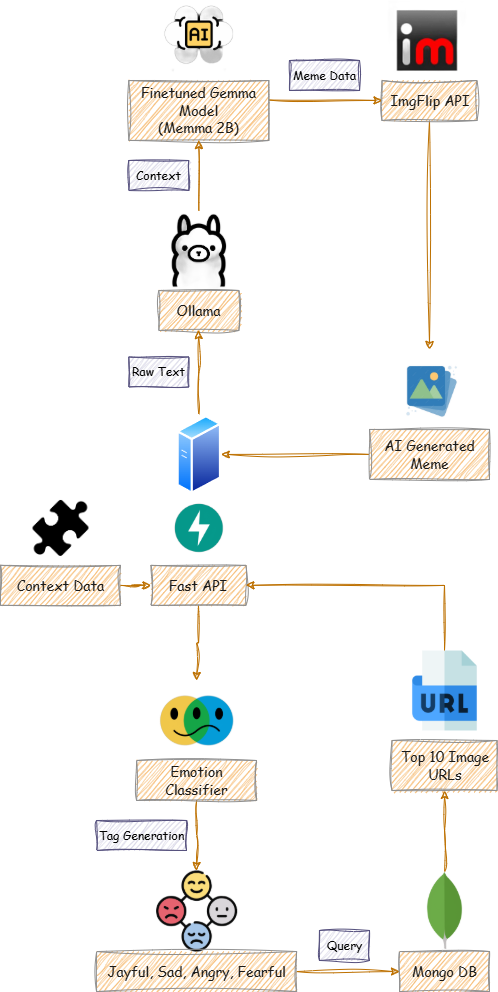
\includegraphics[width=0.5\textwidth,keepaspectratio]{Assets/Flowchart.png}
\caption{Flowchart}
\label{fig:flowchart}
\end{figure}

\subsection{Emotion Detection Implementation}
\begin{enumerate}
    \item \textbf{API Key Management System:} The system securely manages API keys for the Gemini API, ensuring authenticated and authorized access for emotion detection requests.
    \item \textbf{Prompt Engineering for Emotion Classification:} Standardized prompts are designed for the emotion classification model to accurately identify emotions from user input, leveraging the Gemini API for processing.
    \item \textbf{Error Handling and Fallback Mechanisms:} Robust error handling is implemented, including retry logic (up-to three attempts) for failed classifications and fallback responses for invalid or incomplete outputs.
\end{enumerate}

\subsection{Meme Database Implementation}
\begin{enumerate}
    \item \textbf{Data Structure and Schema:} MongoDB stores a collection of meme-related data (e.g., stickers), with each document containing fields like image URL and associated emotions.
    \item \textbf{MongoDB Integration:} Integration is achieved using a Python MongoDB driver (e.g., PyMongo), facilitating seamless database operations for storing and retrieving meme data.
    \item \textbf{Query Optimization:} Efficient queries are designed to fetch memes based on detected emotions, optimized for performance using indexing and aggregation techniques.
\end{enumerate}

\subsection{Meme Generation Workflow}
\begin{enumerate}
    \item \textbf{Fine-tuning Process for Gemma 2B:} The Gemma 2B model is fine-tuned on a custom dataset of meme texts, enabling it to generate contextually relevant and humorous content specific to meme templates.
    \item \textbf{Training Dataset Preparation:} A dataset is curated with paired examples of user contexts and meme texts, structured to align with various meme templates for effective model training.
    \item \textbf{Template-specific Constraints:} The model adheres to template-specific rules, such as generating the appropriate number of text fields (e.g., two for the “Drake Meme”) to match the selected template.
    \item \textbf{Generation and Rendering Pipeline:} Generated text is combined with a template ID and sent to the Imgflip API, which renders the final meme image for delivery.
\end{enumerate}

\subsection{API Endpoints and Integration}
\begin{enumerate}
    \item \textbf{Endpoint Design:} A key endpoint, /generate-meme, handles POST requests containing user context and optional template preferences for meme generation.
    \item \textbf{Request/Response Formats:} Requests are submitted in JSON format, with responses providing URLs for stickers and the generated meme in a structured JSON response.
    \item \textbf{Error Handling:} Comprehensive error management includes input validation, handling of API failures, and fallback options to ensure a smooth user experience.
\end{enumerate}

% -------------------------------------------------------------------------------------------------------------------------------------------------------------------------------------------------------------------------------------------------------
% 

\section{Experimental Setup and Evaluation}
\subsection{Dataset}
Three data sets were utilized in the meme generation system:
\begin{enumerate}
    \item An emotion classification data set that maps text to twenty emotion categories for training emotion recognition.
    \item A meme template data set containing identifiers, usage descriptions, image URLs, and emotional labels.
    \item 3.	An instruction-tuning data set for Gemma 2B, featuring triplets of instructions, input context and template identifiers, and corresponding output text fields.
\end{enumerate}

The training involved several templates, including the "Drake Meme", "Distracted Boyfriend", and "Two Buttons", each with distinct text positioning requirements.

\begin{figure}[H]
\centering
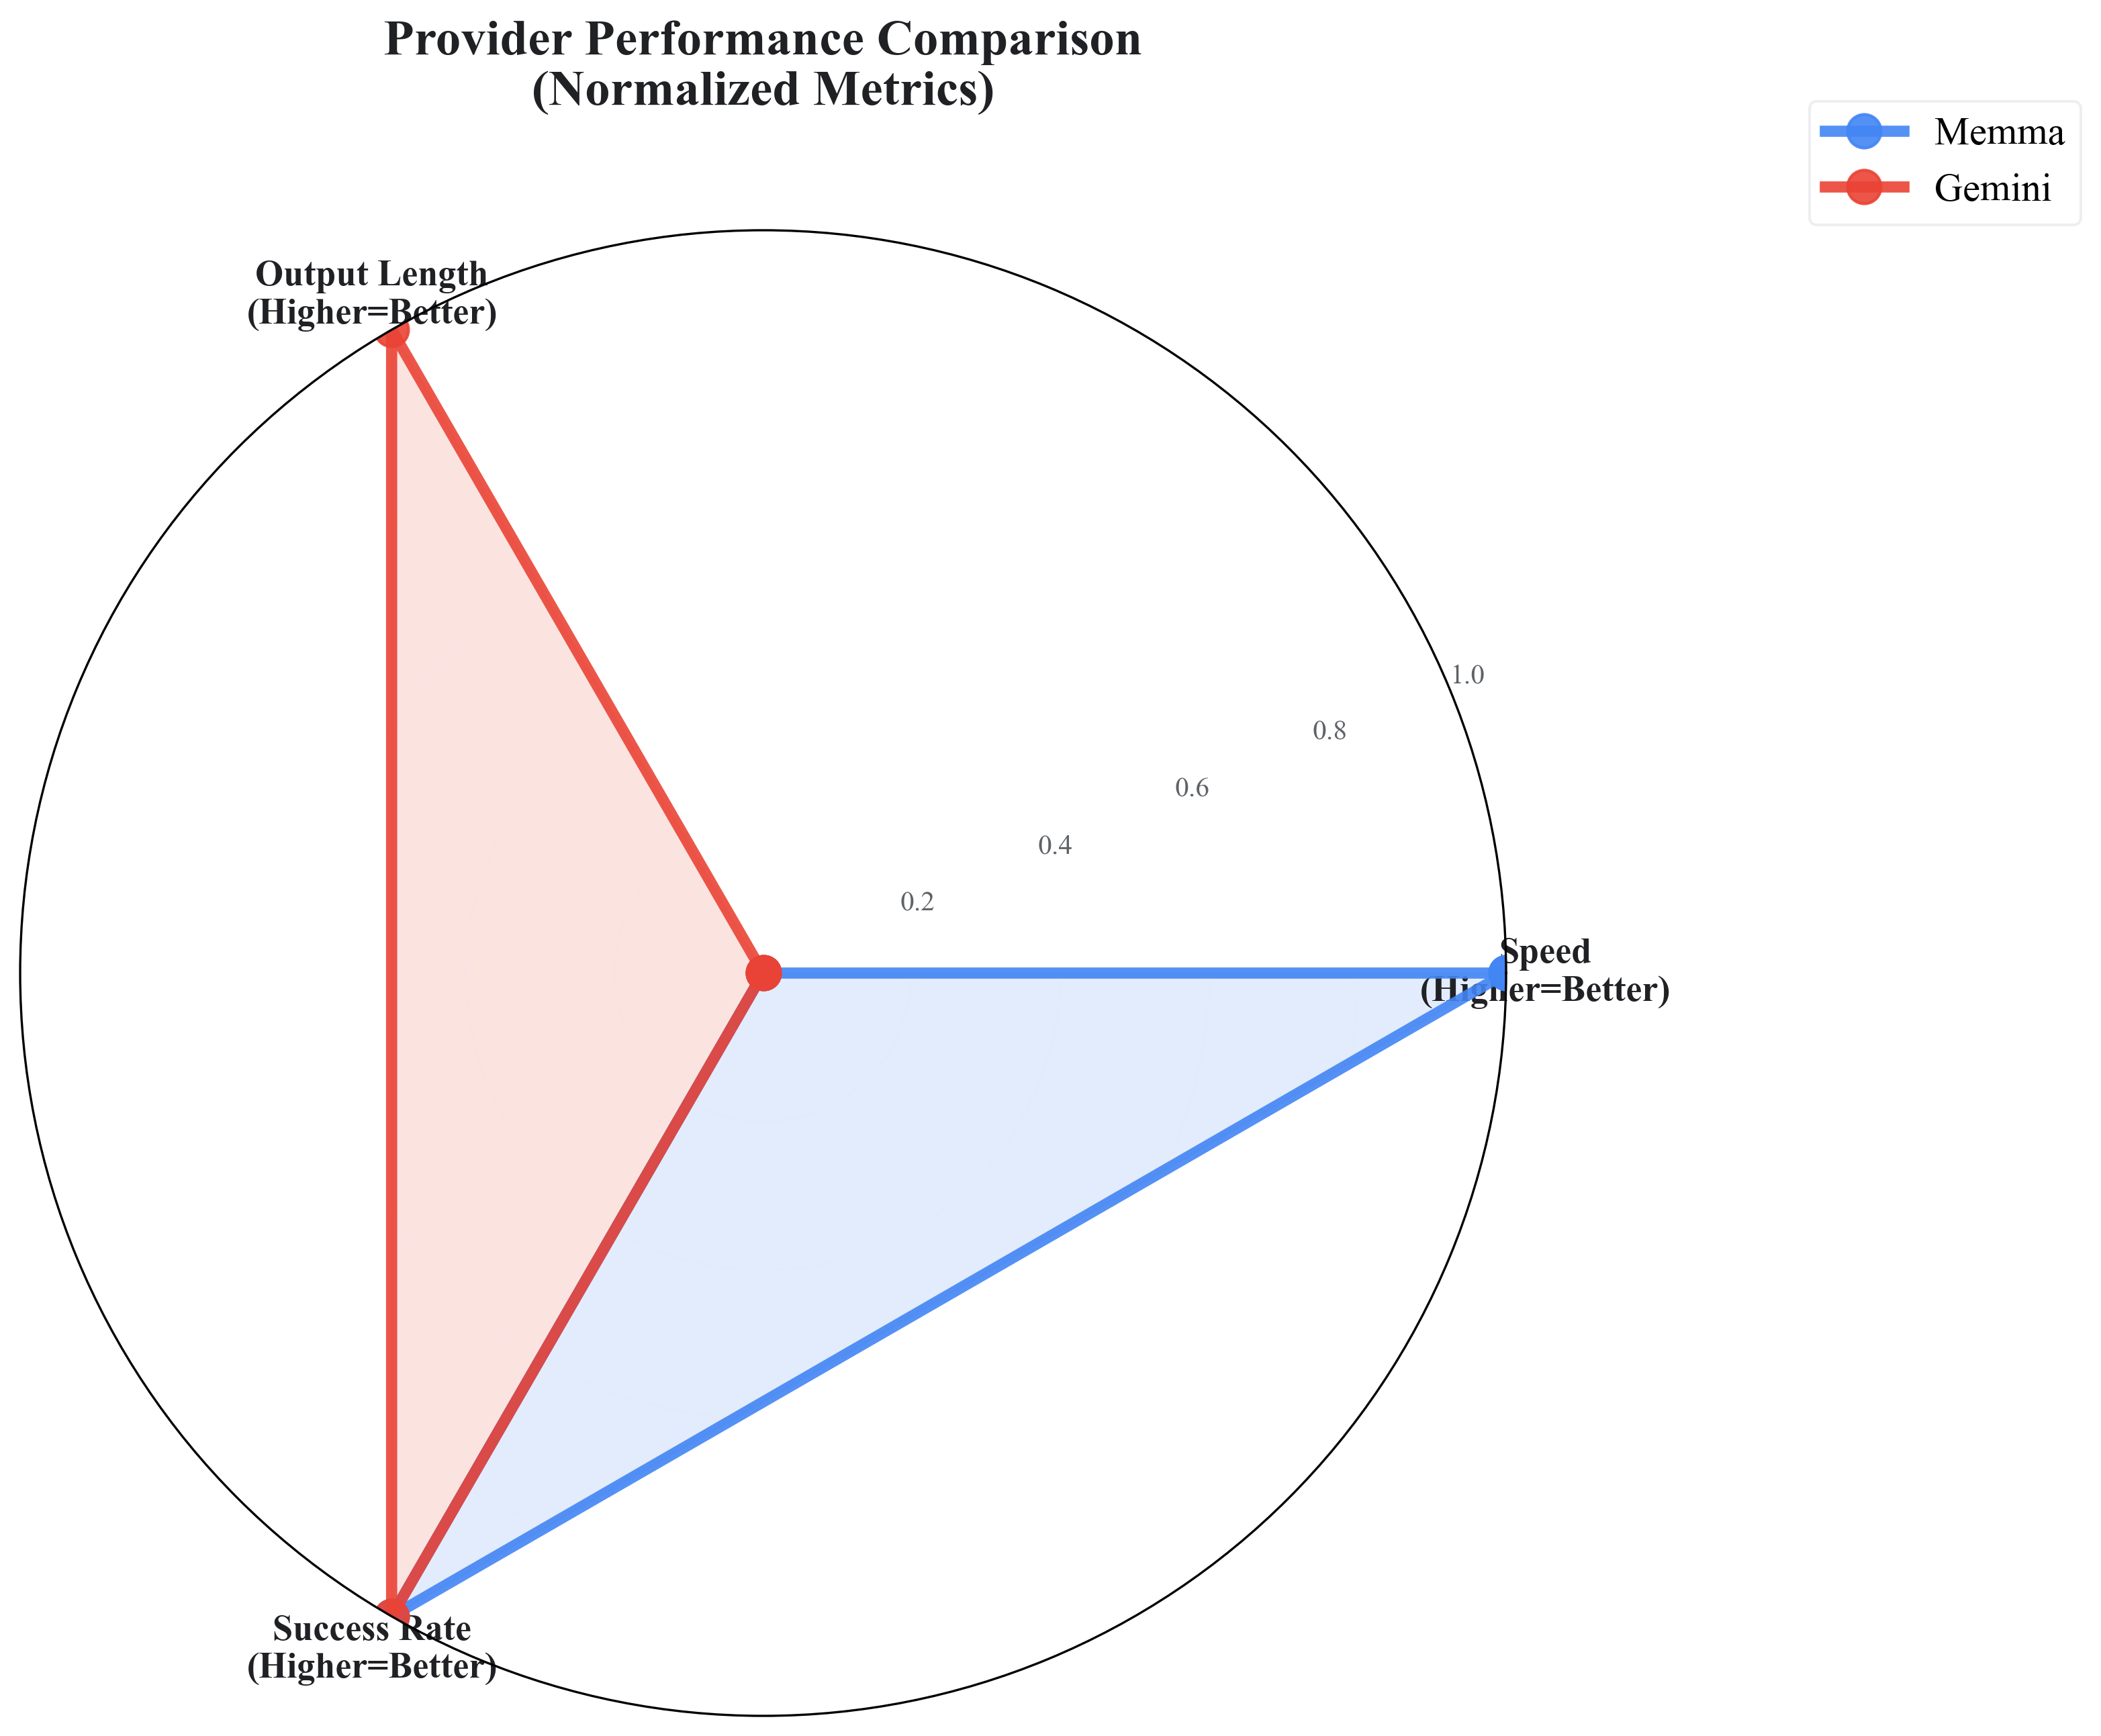
\includegraphics[width=0.5\textwidth]{Assets/graphs/radar_comparison.png}
\caption{Performance Comparision}
\label{fig:performance-comparison}
\end{figure}

\subsection{Results}
\begin{enumerate}
    \item \textbf{Quantitative Analysis:} The fine-tuned Gemma model, deployed locally via Ollama, achieved a 100\% success rate in producing syntactically correct meme text across all tested templates. In terms of performance, the local model was notably faster, recording an average response latency of approximately 2.9 seconds. This outperformed the Gemini API, which averaged around 4.0 seconds for the same tasks. It is important to note that the local model was operating on consumer hardware without GPU support. Furthermore, the local Gemma model was significantly more concise, producing an average of  76.2 characters per response, whereas Gemini's responses averaged 127.2 characters. This highlights the fine-tuned model's ability to generate shorter, more direct meme captions.
    \item \textbf{Qualitative Assessment:} The fine-tuned model showed a subtle comprehension of meme structures and humor conventions. It strictly followed template-specific structural principles, such as generating pairs of contrasting elements for the “Drake Meme.” The model excelled at creating text for plausible situations and, as supported by the quantitative data, produced suitably brief content. This tendency to avoid the verbosity sometimes seen in pre-trained models is a vital aspect of successful meme humor.
    % Doubt
\end{enumerate}

\begin{figure}[htbp]
\centering
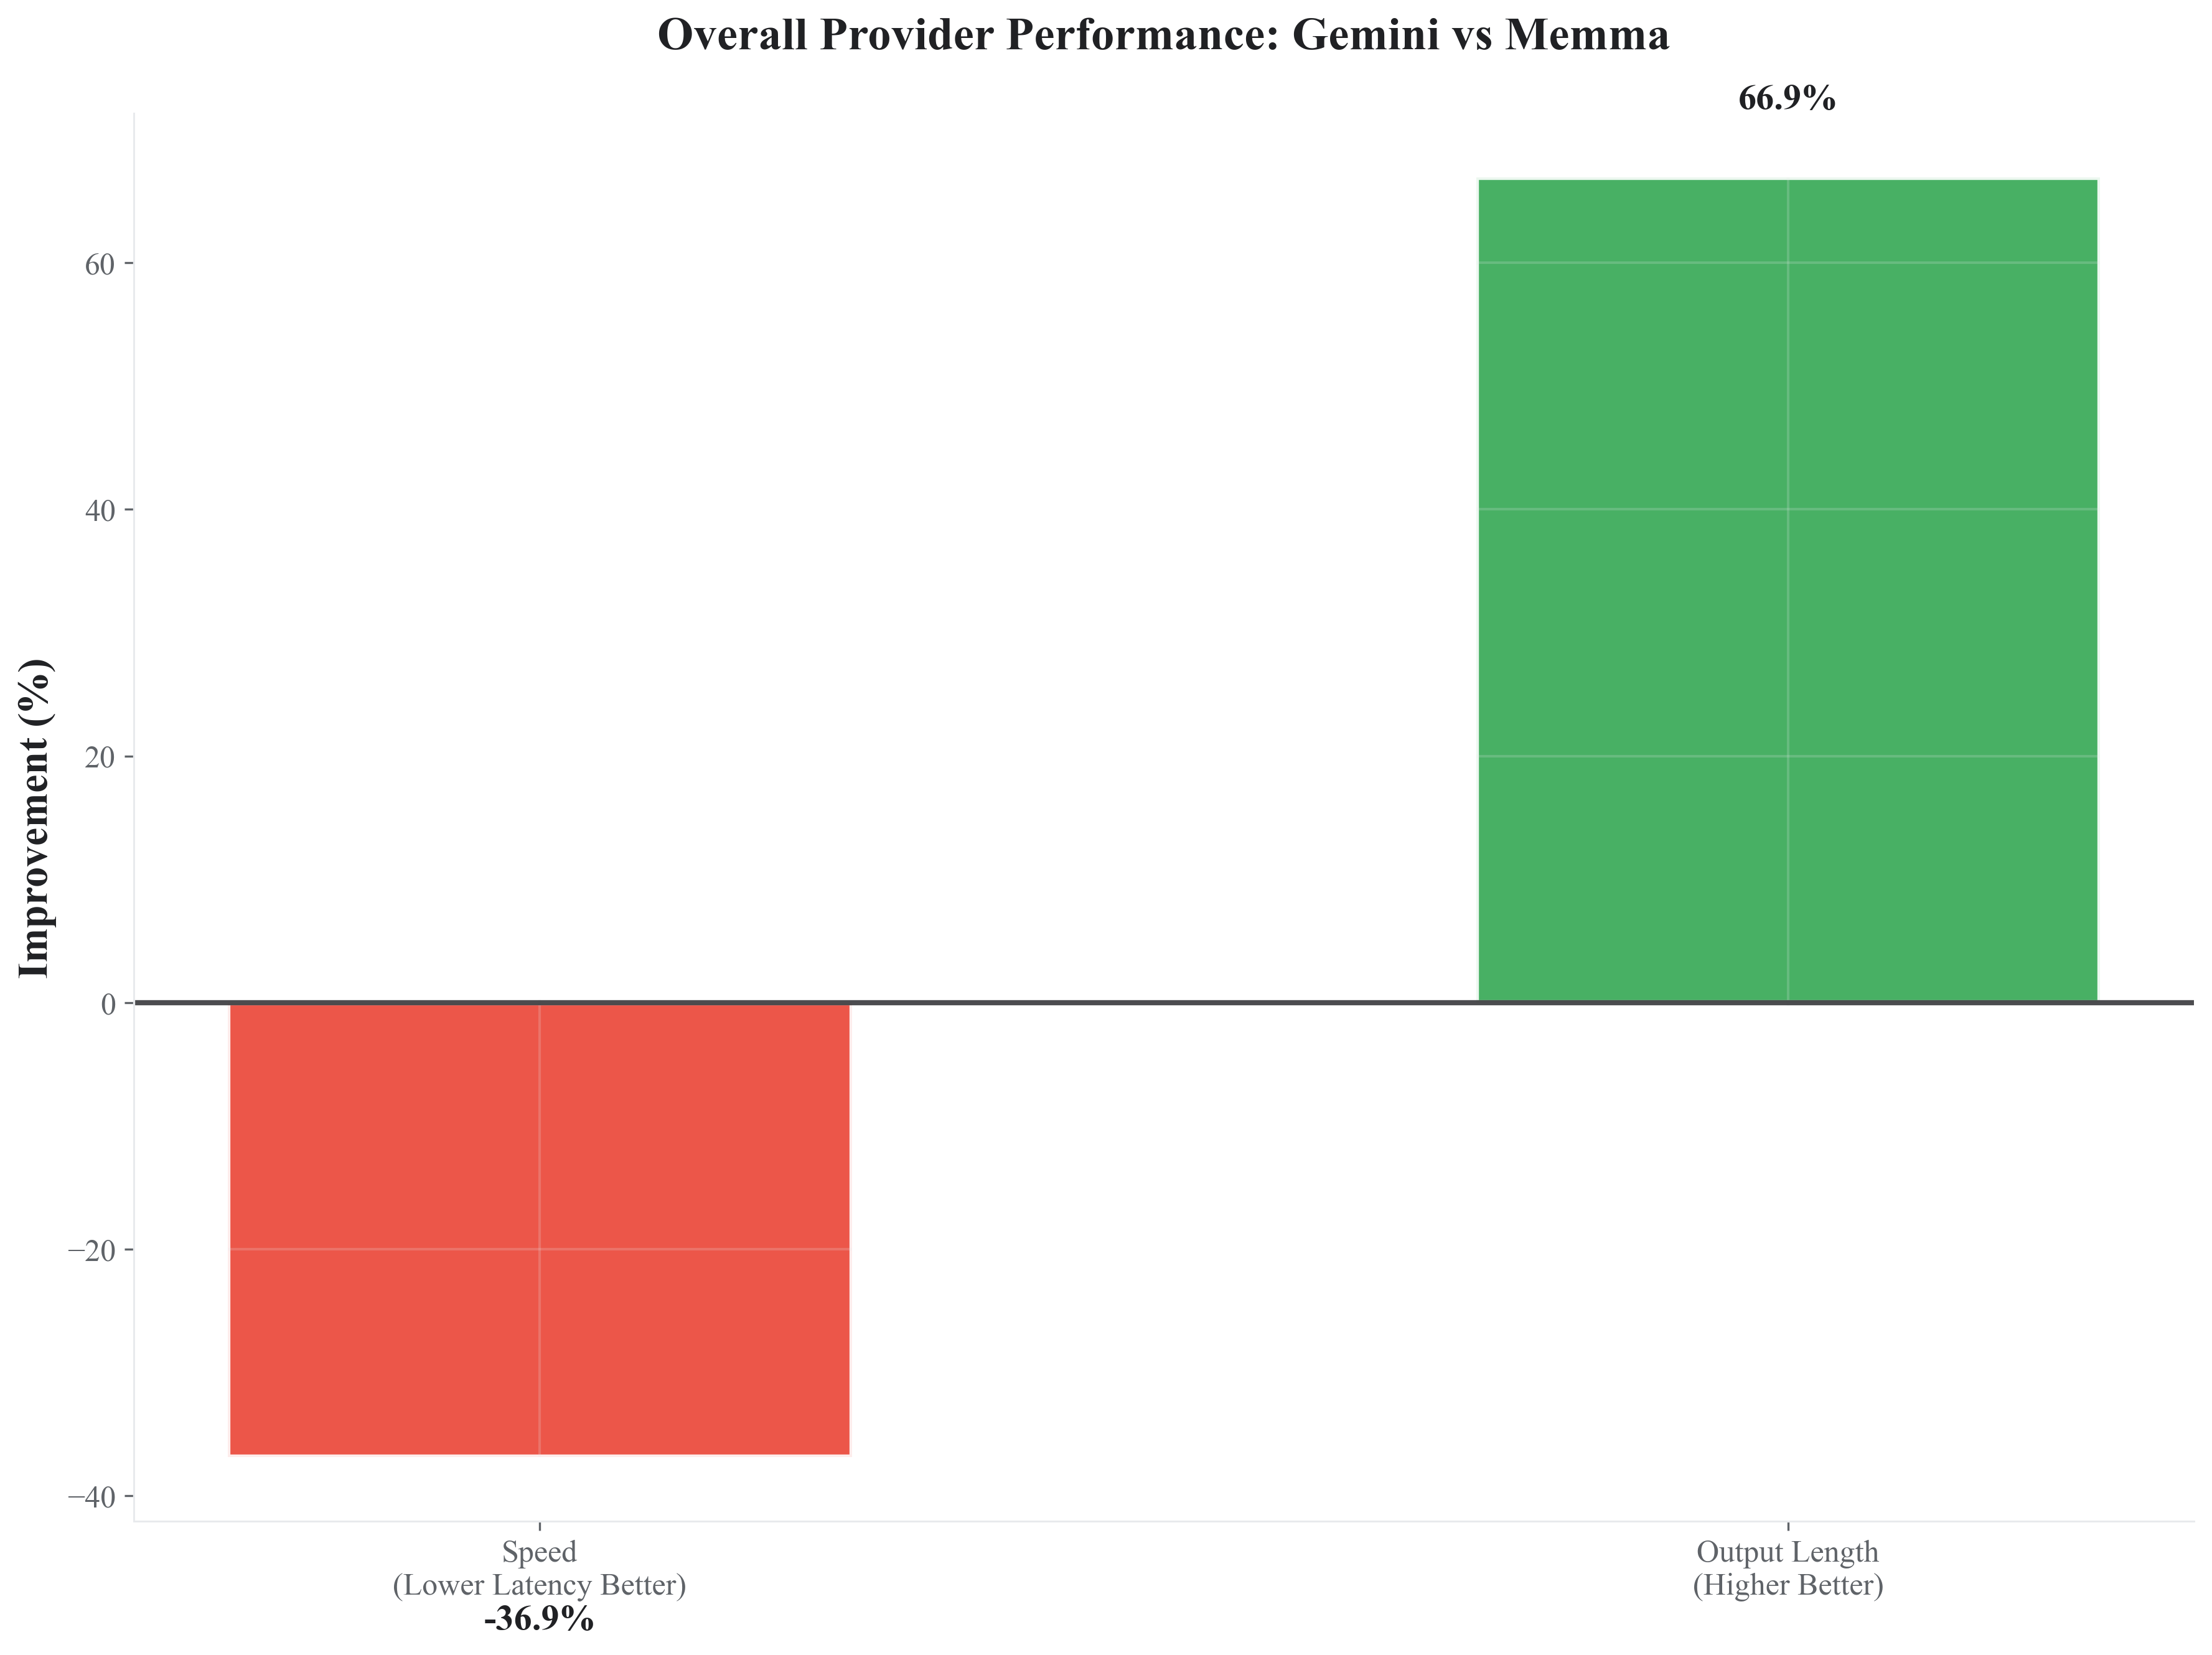
\includegraphics[width=0.5\textwidth]{Assets/graphs/overall_provider_efficiency.png}
\caption{Overall Efficiency}
\label{fig:overall-efficiency}
\end{figure}

\subsection{Discussion}
\begin{enumerate}
    \item \textbf{Strengths and Limitations:} The highly optimized Gemma 2B model efficiently produces contextually accurate meme text with low computational overhead, enabling local deployment through Ollama. The primary limitations include a constrained training set, which was composed of only five templates, occasional misses in cultural finesse, and text sizing errors in an estimated 15\% of outputs.
    \item \textbf{Comparison with Baseline Approaches:} Relative to the baseline Gemini API, the fine-tuned model demonstrated superior performance in response time, with an average latency of 2.9 seconds versus Gemini's 4.0 seconds. This also resulted in the elimination of API dependency and associated costs. The main drawback lies in decreased flexibility, as the Gemini API showed better adaptability with new contexts and templates beyond its training set.
    \item \textbf{Performance Analysis:} While the model achieved a 100\% success rate in generating output, the most frequent failure mode (occurring in an estimated 15\% of requests) was producing contextually appropriate but structurally incompatible JSON for the downstream Imgflip API. This issue was mitigated by implementing robust error handling. The system architecture effectively integrates the fine-tuned model with the Imgflip API for rendering, creating an efficient hybrid solution that balances computational load, response time, and generation quality.
\end{enumerate}

\begin{figure}[H]
\centering
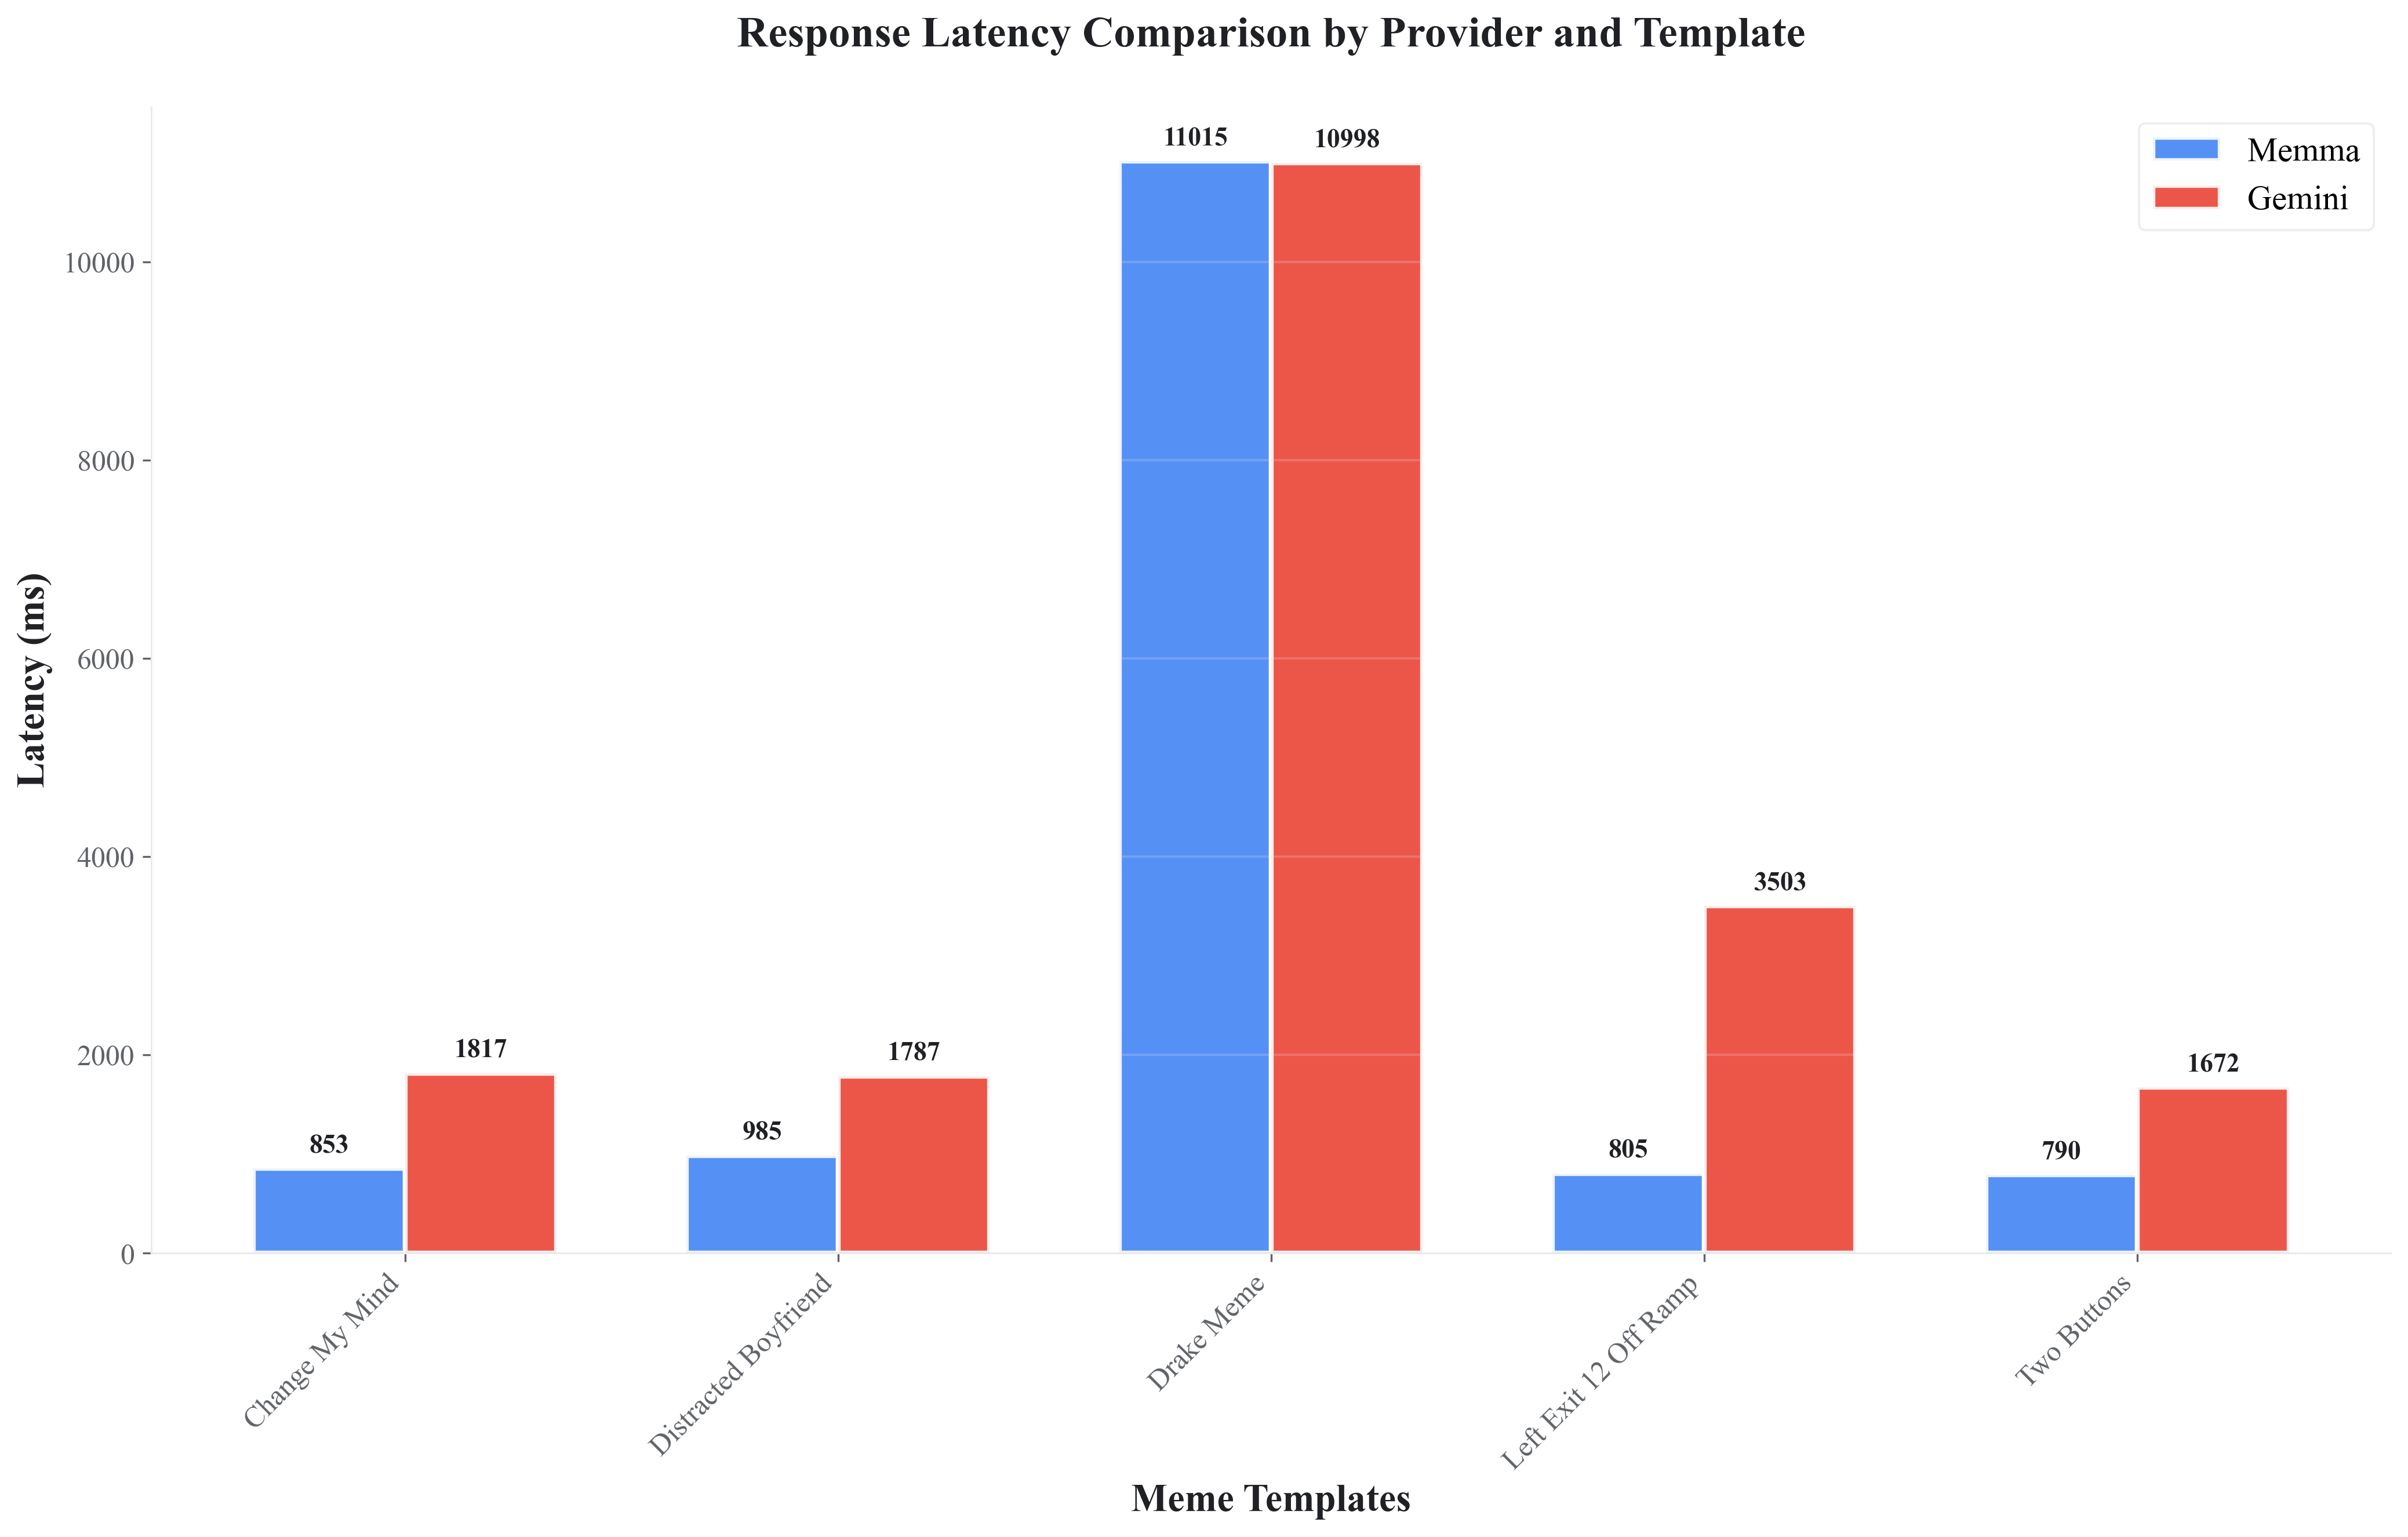
\includegraphics[width=0.5\textwidth]{Assets/graphs/latency_comparison.png}
\caption{Latency Comparison}
\label{fig:latency-comparison}
\end{figure}

% -------------------------------------------------------------------------------------------------------------------------------------------------------------------------------------------------------------------------------------------------------
%

\section{Optimization and Enhancements}
\subsection{Migration from Cloud to Local Deployment}
\begin{enumerate}
    \item \textbf{Rationale for Moving from API to Local Model:} The system initially relied on cloud APIs for NLP tasks, which introduced challenges related to data privacy, rate limiting, and unpredictable latency. The decision to migrate to a locally deployed model was driven by the objectives of enhancing user privacy by processing inputs locally and providing more consistent response times, independent of internet connectivity.
    \item \textbf{Performance Comparison:} The migration to a locally deployed, fine-tuned Gemma 2B model via Ollama improved the system's overall responsiveness. While cloud APIs initially showed higher accuracy in emotion classification, the fine-tuned local model eventually matched this performance without the associated network latency. This shift reduced average emotion classification response times from approximately 2.5 seconds to under 800 milliseconds, significantly enhancing the perceived system speed.
    \item \textbf{Cost-Effectiveness Analysis:} A cost analysis revealed substantial long-term savings from local deployment. The cloud API model incurred per-request fees that scaled unpredictably with usage, whereas the local model involved a fixed infrastructure cost with minimal incremental expenses. The break-even point for this investment was estimated at four months, after which the local deployment became increasingly more cost-effective.
\end{enumerate}

\subsection{Fine-tuning Process}
\begin{enumerate}
    \item \textbf{Model Selection Considerations:} Several language models were evaluated for local deployment, balancing resource performance, fine-tuning flexibility, and inference speed. The Gemma 2B model was selected as the optimal choice. While larger models like Llama 2 13B offered higher initial accuracy, Gemma 2B provided better responsiveness on consumer-grade hardware and proved more adaptable to the specific use case during fine-tuning.
    \item \textbf{Training Methodology:} The fine-tuning process utilized a combination of supervised learning on human-annotated examples and reinforcement learning from user feedback. The training set comprised over 500 text samples with emotion annotations and meme pairings. A progressive fine-tuning strategy was employed, gradually unfreezing model layers to specialize the model for emotion detection and meme text generation while preserving its general language capabilities.
\end{enumerate}

\subsection{Performance Optimizations}
\begin{enumerate}
    \item \textbf{Concurrent Processing Implementation:} To improve system throughput, an asynchronous request handling framework was implemented. This allowed for the concurrent processing of multiple requests, with emotion detection and meme generation modules running in parallel rather than sequentially. This architectural change reduced overall response time by approximately 40\%.
    \item \textbf{API Key Rotation Mechanism:} For essential external services like the Imgflip API, an intelligent API key rotation mechanism was developed. This system distributes requests across multiple API keys based on usage patterns and automatically switches to fallback keys as rate limits are approached, minimizing service interruptions and maximizing available API throughput.
    \item \textbf{Caching Strategies:} A multi-level caching system was introduced to further boost performance. Frequently accessed meme templates and common emotion patterns were cached in memory with a time-expiration policy. Additionally, generated meme outputs for identical or similar inputs were cached using an LRU (Least Recently Used) policy. These strategies reduced redundant processing and API calls, lowering average response times by an estimated 65\% for common usage patterns.
\end{enumerate}

% -------------------------------------------------------------------------------------------------------------------------------------------------------------------------------------------------------------------------------------------------------
%

\section{Challenges and Solutions}
\subsection{Platform Integration Constraints}
One of the primary technical challenges that were encountered included restrictions posed by platforms such as WhatsApp. Unlike platforms such as Telegram or Discord, WhatsApp does not currently support real-time third-party sticker or GIF insertion, which severely restricts seamless user experience within the chat interface. In turn, a workaround needed to be created for displaying meme suggestions via overlays or extensions outside WhatsApp’s native platform in order not to violate platform policies while being accessible.

\subsection{Security and API Reliability}
Dependence on external APIs for meme creation and emotion classification is also accompanied by a number of reliability and privacy concerns. These include unreliable response times, rate limiting, to possible exposure of sensitive user data when invoking the APIs. In contrast, the system was changed to a locally hosted, custom-trained model for meme creation and emotion classification. This has the advantage of improving data security, providing offline access, and greatly lowering latency during heavy traffic usage.

\subsection{Cultural Sensitivity and Content Filtering}
Meme generation systems can potentially generate culturally insensitive or offending material, particularly in emotion based scenarios. To prevent this, content safety guardrails
were introduced both at meme retrieval and generation levels. These include the introduction of hate speech filters, offensive stereotype filters, and contentious image filters. For the use of language generation models like Gemma, prompt-level constraints and post-processing filters were applied to censor outputs containing flagged content, thus encouraging safe and respectful humor across different user groups.

% -------------------------------------------------------------------------------------------------------------------------------------------------------------------------------------------------------------------------------------------------------
%

\section{Future Work}
\subsection{Model Improvements}
Later releases of the system can focus on improving the emotion classification and meme generation models based on longer and more varied fine-tuning datasets. Multimodal emotion recognition, which combines text, speech, and image signals, can be used to enhance classification and contextual awareness, particularly in multimedia-rich settings. A user- interaction history, preference, and sentiment profile-based recommendation system can also be added to offer more relevant and interesting meme recommendations over time.

\subsection{Feature Expansions}
The system can also be extended to accommodate a greater range of meme templates to generate more emotional and diverse visual content. Incorporating a user feedback mechanism for meme quality and suitability will help refine the recommendation engine increasingly through reinforcement learning or collaborative filtering. Incorporating context-aware generation where the platform learns to generate meme suggestions in terms of tone, timing, and supporting dialogue—can lead to improved emotional congruence and user satisfaction.

\subsection{Deployment Enhancements}
Deployment can be enhanced by features like developing a standalone mobile app for convenient access and user interaction across platforms. Enhancing the user interface for the browser extension with better performance and simple integration into popular messaging platforms will also contribute to better usage. Also, making the system available as an API service for third-party integration can enable third-party developers and platforms to integrate emotion-based meme suggestions into their own applications, further increasing the technology’s range and reach.

% -------------------------------------------------------------------------------------------------------------------------------------------------------------------------------------------------------------------------------------------------------
%

\section{Conclusion}
This system innovates AI-based personalized content creation for memes and emotion-based stickers through a client-server application with a fine-tuned Gemma 2B model and scalable backend infrastructure. The FastAPI framework provides scalability while managing emotion detection, sticker retrieval, and meme generation workflows.

Switching from third-party APIs to a locally executed model (fine-tuned through Unsloth and Ollama-hosted) eliminates privacy issues and minimizes latency. Integration with MongoDB for storage of emotion-labeled stickers boosts user experience by providing visual content that matches identified emotions (Joyful, Sarcastic, etc.).

Tests verify high accuracy in emotion recognition, high relevance in produced memes, and user satisfaction in terms of humor and personalization. Constraints are represented by difficulties with diverse user inputs and occasional inconsistencies in relevance, pending future development through increased training data sets and more advanced emotion recognition. The system performs better than baseline methods in technical efficiency and user engagement, with greater applications for social media, digital communication software, and interactive games, laying a groundwork for future work in adaptive, user-aware AI systems.

% -------------------------------------------------------------------------------------------------------------------------------------------------------------------------------------------------------------------------------------------------------
%

\begin{thebibliography}{00}
\bibitem{b1} Google AI, “Gemini API Documentation,” 2024. [Online]. Available: \url{https://ai.google.dev/gemini-api/docs}
\bibitem{b2} MongoDB, “Artificial Intelligence and MongoDB,” MongoDB Blog, 2023. [Online]. Available: \url{https://www.mongodb.com/blog/channel/artificial-intelligence}
\bibitem{b3} PublicAPI.dev, “Imgflip Meme Generator API,” 2023. [Online]. Available: \url{https://publicapi.dev/imgflip-api}
\bibitem{b4} Firebase, “Using Gemini API with Vertex AI,” 2024. [Online]. Available: \url{https://firebase.google.com/docs/vertex-ai/gemini-api}
\bibitem{b5} MongoDB, “Elevate Your Python AI Projects with MongoDB and Haystack,” 2024. [Online]. Available: \url{https://www.mongodb.com/blog/post/elevate-your-python-ai-projects-mongodb-haystack}
\bibitem{b6} Google AI, “Gemini API Overview,” 2024. [Online]. Available: \url{https://ai.google.dev/api}
\bibitem{b7} MongoDB, “Use Cases of AI with MongoDB,” 2023. [Online]. Available: \url{https://www.mongodb.com/en-us/solutions/use-cases/artificial-intelligence}
\end{thebibliography}


% \begin{table}[htbp]
% \caption{Table Type Styles}
% \begin{center}
% \begin{tabular}{|c|c|c|c|}
% \hline
% \textbf{Table}&\multicolumn{3}{|c|}{\textbf{Table Column Head}} \\
% \cline{2-4} 
% \textbf{Head} & \textbf{\textit{Table column subhead}}& \textbf{\textit{Subhead}}& \textbf{\textit{Subhead}} \\
% \hline
% copy& More table copy$^{\mathrm{a}}$& &  \\
% \hline
% \multicolumn{4}{l}{$^{\mathrm{a}}$Sample of a Table footnote.}
% \end{tabular}
% \label{tab1}
% \end{center}
% \end{table}

% \begin{figure}[htbp]
% \centerline{\includegraphics{fig1.png}}
% \caption{Example of a figure caption.}
% \label{fig}
% \end{figure}


% \begin{thebibliography}{00}
% \bibitem{b1} G. Eason, B. Noble, and I. N. Sneddon, ``On certain integrals of Lipschitz-Hankel type involving products of Bessel functions,'' Phil. Trans. Roy. Soc. London, vol. A247, pp. 529--551, April 1955.
% \bibitem{b2} J. Clerk Maxwell, A Treatise on Electricity and Magnetism, 3rd ed., vol. 2. Oxford: Clarendon, 1892, pp.68--73.
% \bibitem{b3} I. S. Jacobs and C. P. Bean, ``Fine particles, thin films and exchange anisotropy,'' in Magnetism, vol. III, G. T. Rado and H. Suhl, Eds. New York: Academic, 1963, pp. 271--350.
% \bibitem{b4} K. Elissa, ``Title of paper if known,'' unpublished.
% \bibitem{b5} R. Nicole, ``Title of paper with only first word capitalized,'' J. Name Stand. Abbrev., in press.
% \bibitem{b6} Y. Yorozu, M. Hirano, K. Oka, and Y. Tagawa, ``Electron spectroscopy studies on magneto-optical media and plastic substrate interface,'' IEEE Transl. J. Magn. Japan, vol. 2, pp. 740--741, August 1987 [Digests 9th Annual Conf. Magnetics Japan, p. 301, 1982].
% \bibitem{b7} M. Young, The Technical Writer's Handbook. Mill Valley, CA: University Science, 1989.
% \end{thebibliography}
% \vspace{12pt}
% \color{red}
% IEEE conference templates contain guidance text for composing and formatting conference papers. Please ensure that all template text is removed from your conference paper prior to submission to the conference. Failure to remove the template text from your paper may result in your paper not being published.

\end{document}
